
%% bare_adv.tex
%% V1.3
%% 2007/01/11
%% by Michael Shell
%% See: 
%% http://www.michaelshell.org/
%% for current contact information.
%%
%% This is a skeleton file demonstrating the advanced use of IEEEtran.cls
%% (requires IEEEtran.cls version 1.7 or later) with an IEEE Computer
%% Society journal paper.
%%
%% Support sites:
%% http://www.michaelshell.org/tex/ieeetran/
%% http://www.ctan.org/tex-archive/macros/latex/contrib/IEEEtran/
%% and
%% http://www.ieee.org/

%%*************************************************************************
%% Legal Notice:
%% This code is offered as-is without any warranty either expressed or
%% implied; without even the implied warranty of MERCHANTABILITY or
%% FITNESS FOR A PARTICULAR PURPOSE! 
%% User assumes all risk.
%% In no event shall IEEE or any contributor to this code be liable for
%% any damages or losses, including, but not limited to, incidental,
%% consequential, or any other damages, resulting from the use or misuse
%% of any information contained here.
%%
%% All comments are the opinions of their respective authors and are not
%% necessarily endorsed by the IEEE.
%%
%% This work is distributed under the LaTeX Project Public License (LPPL)
%% ( http://www.latex-project.org/ ) version 1.3, and may be freely used,
%% distributed and modified. A copy of the LPPL, version 1.3, is included
%% in the base LaTeX documentation of all distributions of LaTeX released
%% 2003/12/01 or later.
%% Retain all contribution notices and credits.
%% ** Modified files should be clearly indicated as such, including  **
%% ** renaming them and changing author support contact information. **
%%
%% File list of work: IEEEtran.cls, IEEEtran_HOWTO.pdf, bare_adv.tex,
%%                    bare_conf.tex, bare_jrnl.tex, bare_jrnl_compsoc.tex
%%*************************************************************************

% *** Authors should verify (and, if needed, correct) their LaTeX system  ***
% *** with the testflow diagnostic prior to trusting their LaTeX platform ***
% *** with production work. IEEE's font choices can trigger bugs that do  ***
% *** not appear when using other class files.                            ***
% The testflow support page is at:
% http://www.michaelshell.org/tex/testflow/



% IEEEtran V1.7 and later provides for these CLASSINPUT macros to allow the
% user to reprogram some IEEEtran.cls defaults if needed. These settings
% override the internal defaults of IEEEtran.cls regardless of which class
% options are used. Do not use these unless you have good reason to do so as
% they can result in nonIEEE compliant documents. User beware. ;)
%
%\newcommand{\CLASSINPUTbaselinestretch}{1.0} % baselinestretch
%\newcommand{\CLASSINPUTinnersidemargin}{1in} % inner side margin
%\newcommand{\CLASSINPUToutersidemargin}{1in} % outer side margin
%\newcommand{\CLASSINPUTtoptextmargin}{1in}   % top text margin
%\newcommand{\CLASSINPUTbottomtextmargin}{1in}% bottom text margin



% Note that the a4paper option is mainly intended so that authors in
% countries using A4 can easily print to A4 and see how their papers will
% look in print - the typesetting of the document will not typically be
% affected with changes in paper size (but the bottom and side margins will).
% Use the testflow package mentioned above to verify correct handling of
% both paper sizes by the user's LaTeX system.
%
% Also note that the "draftcls" or "draftclsnofoot", not "draft", option
% should be used if it is desired that the s are to be displayed in
% draft mode.
%
\documentclass[10pt,journal,a4paper]{IEEEtran}
% If IEEEtran.cls has not been installed into the LaTeX system files,
% manually specify the path to it like:
% \documentclass[10pt,journal,compsoc]{../sty/IEEEtran}


% For Computer Society journals, IEEEtran defaults to the use of 
% Palatino/Palladio as is done in IEEE Computer Society journals.
% To go back to Times Roman, you can use this code:
%\renewcommand{\rmdefault}{ptm}\selectfont





% Some very useful LaTeX packages include:
% (uncomment the ones you want to load)



% *** MISC UTILITY PACKAGES ***
%
%\usepackage{ifpdf}
% Heiko Oberdiek's ifpdf.sty is very useful if you need conditional
% compilation based on whether the output is pdf or dvi.
% usage:
% \ifpdf
%   % pdf code
% \else
%   % dvi code
% \fi
% The latest version of ifpdf.sty can be obtained from:
% http://www.ctan.org/tex-archive/macros/latex/contrib/oberdiek/
% Also, note that IEEEtran.cls V1.7 and later provides a builtin
% \ifCLASSINFOpdf conditional that works the same way.
% When switching from latex to pdflatex and vice-versa, the compiler may
% have to be run twice to clear warning/error messages.






% *** CITATION PACKAGES ***
%
\ifCLASSOPTIONcompsoc
  % IEEE Computer Society needs nocompress option
  % requires cite.sty v4.0 or later (November 2003)
  % \usepackage[nocompress]{cite}
\else
  % normal IEEE
  % \usepackage{cite}
\fi
% cite.sty was written by Donald Arseneau
% V1.6 and later of IEEEtran pre-defines the format of the cite.sty package
% \cite{} output to follow that of IEEE. Loading the cite package will
% result in citation numbers being automatically sorted and properly
% "compressed/ranged". e.g., [1], [9], [2], [7], [5], [6] without using
% cite.sty will become [1], [2], [5]--[7], [9] using cite.sty. cite.sty's
% \cite will automatically add leading space, if needed. Use cite.sty's
% noadjust option (cite.sty V3.8 and later) if you want to turn this off.
% cite.sty is already installed on most LaTeX systems. Be sure and use
% version 4.0 (2003-05-27) and later if using hyperref.sty. cite.sty does
% not currently provide for hyperlinked citations.
% The latest version can be obtained at:
% http://www.ctan.org/tex-archive/macros/latex/contrib/cite/
% The documentation is contained in the cite.sty file itself.
%
% Note that some packages require special options to format as the Computer
% Society requires. In particular, Computer Society  papers do not use
% compressed citation ranges as is done in typical IEEE papers
% (e.g., [1]-[4]). Instead, they list every citation separately in order
% (e.g., [1], [2], [3], [4]). To get the latter we need to load the cite
% package with the nocompress option which is supported by cite.sty v4.0
% and later. Note also the use of a CLASSOPTION conditional provided by
% IEEEtran.cls V1.7 and later.





% *** GRAPHICS RELATED PACKAGES ***
%
\ifCLASSINFOpdf
  % \usepackage[pdftex]{graphicx}
  % declare the path(s) where your graphic files are
  % \graphicspath{{../pdf/}{../jpeg/}}
  % and their extensions so you won't have to specify these with
  % every instance of \includegraphics
  % \DeclareGraphicsExtensions{.pdf,.jpeg,.png}
\else
  % or other class option (dvipsone, dvipdf, if not using dvips). graphicx
  % will default to the driver specified in the system graphics.cfg if no
  % driver is specified.
  % \usepackage[dvips]{graphicx}
  % declare the path(s) where your graphic files are
  % \graphicspath{{../eps/}}
  % and their extensions so you won't have to specify these with
  % every instance of \includegraphics
  % \DeclareGraphicsExtensions{.eps}
\fi
% graphicx was written by David Carlisle and Sebastian Rahtz. It is
% required if you want graphics, photos, etc. graphicx.sty is already
% installed on most LaTeX systems. The latest version and documentation can
% be obtained at: 
% http://www.ctan.org/tex-archive/macros/latex/required/graphics/
% Another good source of documentation is "Using Imported Graphics in
% LaTeX2e" by Keith Reckdahl which can be found as epslatex.ps or
% epslatex.pdf at: http://www.ctan.org/tex-archive/info/
%
% latex, and pdflatex in dvi mode, support graphics in encapsulated
% postscript (.eps) format. pdflatex in pdf mode supports graphics
% in .pdf, .jpeg, .png and .mps (metapost) formats. Users should ensure
% that all non-photo figures use a vector format (.eps, .pdf, .mps) and
% not a bitmapped formats (.jpeg, .png). IEEE frowns on bitmapped formats
% which can result in "jaggedy"/blurry rendering of lines and letters as
% well as large increases in file sizes.
%
% You can find documentation about the pdfTeX application at:
% http://www.tug.org/applications/pdftex


%\usepackage{ps4pdf}
% dvi->ps workflow is required to use such packages as psfrag.sty and
% pstricks.sty. However, Rolf Niepraschk's ps4pdf.sty provides a way to
% apply psfrag/pstricks effects to .eps figures and then get the resultant
% figures in .pdf form. Thus, providing an easier way for migrating from
% .eps to .pdf figures. After ps4pdf.sty loads, if:
% 1. producing .dvi output: the output file will consist ONLY of the
%    figures (or other constructs encased within \PSforPDF commands)
% 2. producing .pdf output: pdflatex will look in the filename-pics.pdf
%    file, where filename is the basename of the tex document, for the
%    graphics (or other constructs encased within \PSforPDF commands).
%    NOTE: If you ever change your figures, you must remember to remake
%    the filename-pics.pdf file.
%
% This way you can do a:
% 
% latex filename
% dvips -Ppdf -o filename-pics.ps filename.dvi
% ps2pdf filename-pics.ps filename-pics.pdf
% 
% to produce a filename-pics.pdf graphics container that contains
% .pdf versions of the graphics with psfrag, pstricks, etc. features.
% Note that you will not typically be able to view the figures in 
% filename-pics.ps because of an offset. However, you will be able to
% view them in filename-pics.pdf. Also, note that when ps4pdf is in effect
% with .dvi output, you may get harmless over/under full box warnings - 
% ignore them. 
% Then, run pdflatex:
% 
% pdflatex filename
% 
% to use pdflatex to make PDF output, automatically using the figures in
% filename-pics.pdf. Alternatively, you could use dvips -i option to
% obtain separate .pdf files for each figure:
%
% dvips -Ppdf -i -E -o fig filename
%
% then convert each figure to pdf via a command such as epstopdf and then
% use pdflatex with these pdf figures and then to dispense with ps4pdf.
%
% Remember to rerun through latex/dvips/ps2pdf if you ever change your
% figures so that filename-pics.pdf gets updated.
% ps4pdf requires David Kastrup's preview-latex and a recent LaTeX system
% (circa 2001 or later). The ps4pdf package and documentation can be
% obtained at: http://www.ctan.org/tex-archive/macros/latex/contrib/ps4pdf/
% The preview-latex package and documentation can be obtained at:
% http://www.ctan.org/tex-archive/macros/latex/contrib/preview/
%
% provide a bogus \PSforPDF, even when not loading pd4pdf. This way we can
% stop loading ps4pdf.sty if we choose to make separate .pdf versions of
% each of our figures.
\providecommand{\PSforPDF}[1]{#1}
% Note that in order for ps4pdf to work, all commands related to psfrag,
% pstricks, etc. must be called within the PSforPDF command. This applies
% even when *loading* via \usepackage psfrag.sty, etc.

\usepackage{graphicx}
%\PSforPDF{\usepackage{psfrag}}
% psfrag.sty was written by Craig Barratt, Michael C. Grant, and
% David Carlisle. It allows you to substitute LaTeX commands for text in
% imported EPS graphic files. In this way, LaTeX symbols can be placed into
% graphics that have been generated by other applications. You must use
% latex->dvips->ps2pdf workflow (not direct pdf output from pdflatex) if
% you wish to use this capability because it works via some PostScript
% tricks. Alternatively, the graphics could be processed as separate files
% via psfrag and dvips, then converted to PDF for inclusion in the main file
% which uses pdflatex. ps4pdf.sty (above) provides a way of doing this all
% at once within the main file.
% Docs are in "The PSfrag System" by Michael C. Grant and David Carlisle.
% There is also some information about using psfrag in "Using Imported
% Graphics in LaTeX2e" by Keith Reckdahl which documents the graphicx
% package (see above). The psfrag package and documentation can be obtained
% at: http://www.ctan.org/tex-archive/macros/latex/contrib/psfrag/
% 
% Note that the current version of psfrag does not "turn itself off" when
% running under pdf output. This will result in a harmless warning
% about a non-PDF \special. However, to silence this, a bogus psfrag
% command can be provided instead of loading psfrag.sty when PDF output
% is being used. Thus, a more complex alternative conditional loading scheme
% can be employed instead of the straightforword way above:
%
%\ifCLASSINFOpdf
% if outputting PDF, do not use or load psfrag.sty as current versions
% output a non-PDF special that generates a harmless, but annoying warning.
% Instead, we provide a bogus \psfrag command that does nothing with
% its arguments. This is a tad tricky because \psfrag can have up to six
% arguments four of which are optional: \psfrag{}[][][][]{}
% Code based on that in psfrag.sty
%\makeatletter
%\def\psfrag{\@ifstar{\@BOGUSpsfraga}{\@BOGUSpsfraga}}
%\def\@BOGUSpsfraga{\begingroup
%   \@makeother\"\@makeother\*\@makeother\!\@makeother\~%
%   \@makeother\:\@makeother\\\@makeother\%\@makeother\#%
%   \@makeother\ \@BOGUSpsfragb}
%\def\@BOGUSpsfragb#1{\endgroup
%                \@ifnextchar [{\@BOGUSpsfragc}%
%                              {\@BOGUSpsfrag}}
%\def\@BOGUSpsfragc[#1]{\@ifnextchar [{\@BOGUSpsfragd}%
%                                     {\@BOGUSpsfrag}}
%\def\@BOGUSpsfragd[#1]{\@ifnextchar [{\@BOGUSpsfrage}%
%                                     {\@BOGUSpsfrag}}
%\def\@BOGUSpsfrage[#1]{\@ifnextchar [{\@BOGUSpsfragf}%
%                                     {\@BOGUSpsfrag}}
%\def\@BOGUSpsfragf[#1]{\@BOGUSpsfrag}
%\def\@BOGUSpsfrag#1{\ignorespaces}
%\makeatother
%\else
% using dvi output, load psfrag, but funnel it through PSforPDF
% as required by ps4pdf.sty
%\PSforPDF{\usepackage{psfrag}}
%\fi





% *** MATH PACKAGES ***
%
%\usepackage[cmex10]{amsmath}
% A popular package from the American Mathematical Society that provides
% many useful and powerful commands for dealing with mathematics. If using
% it, be sure to load this package with the cmex10 option to ensure that
% only type 1 fonts will utilized at all point sizes. Without this option,
% it is possible that some math symbols, particularly those within
% footnotes, will be rendered in bitmap form which will result in a
% document that can not be IEEE Xplore compliant!
%
% Also, note that the amsmath package sets \interdisplaylinepenalty to 10000
% thus preventing page breaks from occurring within multiline equations. Use:
%\interdisplaylinepenalty=2500
% after loading amsmath to restore such page breaks as IEEEtran.cls normally
% does. amsmath.sty is already installed on most LaTeX systems. The latest
% version and documentation can be obtained at:
% http://www.ctan.org/tex-archive/macros/latex/required/amslatex/math/





% *** SPECIALIZED LIST PACKAGES ***
%\usepackage{acronym}
% acronym.sty was written by Tobias Oetiker. This package provides tools for
% managing documents with large numbers of acronyms. (You don't *have* to
% use this package - unless you have a lot of acronyms, you may feel that
% such package management of them is bit of an overkill.)
% Do note that the acronym environment (which lists acronyms) will have a
% problem when used under IEEEtran.cls because acronym.sty relies on the
% description list environment - which IEEEtran.cls has customized for
% producing IEEE style lists. A workaround is to declared the longest
% label width via the IEEEtran.cls \IEEEiedlistdecl global control:
%
% \renewcommand{\IEEEiedlistdecl}{\IEEEsetlabelwidth{SONET}}
% \begin{acronym}
%
% \end{acronym}
% \renewcommand{\IEEEiedlistdecl}{\relax}% remember to reset \IEEEiedlistdecl
%
% instead of using the acronym environment's optional argument.
% The latest version and documentation can be obtained at:
% http://www.ctan.org/tex-archive/macros/latex/contrib/acronym/


%\usepackage{algorithmic}
% algorithmic.sty was written by Peter Williams and Rogerio Brito.
% This package provides an algorithmic environment fo describing algorithms.
% You can use the algorithmic environment in-text or within a figure
% environment to provide for a floating algorithm. Do NOT use the algorithm
% floating environment provided by algorithm.sty (by the same authors) or
% algorithm2e.sty (by Christophe Fiorio) as IEEE does not use dedicated
% algorithm float types and packages that provide these will not provide
% correct IEEE style captions. The latest version and documentation of
% algorithmic.sty can be obtained at:
% http://www.ctan.org/tex-archive/macros/latex/contrib/algorithms/
% There is also a support site at:
% http://algorithms.berlios.de/index.html
% Also of interest may be the (relatively newer and more customizable)
% algorithmicx.sty package by Szasz Janos:
% http://www.ctan.org/tex-archive/macros/latex/contrib/algorithmicx/




% *** ALIGNMENT PACKAGES ***
%
%\usepackage{array}
% Frank Mittelbach's and David Carlisle's array.sty patches and improves
% the standard LaTeX2e array and tabular environments to provide better
% appearance and additional user controls. As the default LaTeX2e table
% generation code is lacking to the point of almost being broken with
% respect to the quality of the end results, all users are strongly
% advised to use an enhanced (at the very least that provided by array.sty)
% set of table tools. array.sty is already installed on most systems. The
% latest version and documentation can be obtained at:
% http://www.ctan.org/tex-archive/macros/latex/required/tools/


%\usepackage{mdwmath}
%\usepackage{mdwtab}
% Also highly recommended is Mark Wooding's extremely powerful MDW tools,
% especially mdwmath.sty and mdwtab.sty which are used to format equations
% and tables, respectively. The MDWtools set is already installed on most
% LaTeX systems. The lastest version and documentation is available at:
% http://www.ctan.org/tex-archive/macros/latex/contrib/mdwtools/


% IEEEtran contains the IEEEeqnarray family of commands that can be used to
% generate multiline equations as well as matrices, tables, etc., of high
% quality.


%\usepackage{eqparbox}
% Also of notable interest is Scott Pakin's eqparbox package for creating
% (automatically sized) equal width boxes - aka "natural width parboxes".
% Available at:
% http://www.ctan.org/tex-archive/macros/latex/contrib/eqparbox/





% *** SUBFIGURE PACKAGES ***
%\ifCLASSOPTIONcompsoc
%\usepackage[tight,normalsize,sf,SF]{subfigure}
%\else
%\usepackage[tight,footnotesize]{subfigure}
%\fi
% subfigure.sty was written by Steven Douglas Cochran. This package makes it
% easy to put subfigures in your figures. e.g., "Figure 1a and 1b". For IEEE
% work, it is a good idea to load it with the tight package option to reduce
% the amount of white space around the subfigures. Computer Society papers
% use a larger font and \sffamily font for their captions, hence the
% additional options needed under compsoc mode. subfigure.sty is already
% installed on most LaTeX systems. The latest version and documentation can
% be obtained at:
% http://www.ctan.org/tex-archive/obsolete/macros/latex/contrib/subfigure/
% subfigure.sty has been superceeded by subfig.sty.


%\ifCLASSOPTIONcompsoc
%  \usepackage[caption=false]{caption}
%  \usepackage[font=normalsize,labelfont=sf,textfont=sf]{subfig}
%\else
%  \usepackage[caption=false]{caption}
%  \usepackage[font=footnotesize]{subfig}
%\fi
% subfig.sty, also written by Steven Douglas Cochran, is the modern
% replacement for subfigure.sty. However, subfig.sty requires and
% automatically loads Axel Sommerfeldt's caption.sty which will override
% IEEEtran.cls handling of captions and this will result in nonIEEE style
% figure/table captions. To prevent this problem, be sure and preload
% caption.sty with its "caption=false" package option. This is will preserve
% IEEEtran.cls handing of captions. Version 1.3 (2005/06/28) and later 
% (recommended due to many improvements over 1.2) of subfig.sty supports
% the caption=false option directly:
%\ifCLASSOPTIONcompsoc
%  \usepackage[caption=false,font=normalsize,labelfont=sf,textfont=sf]{subfig}
%\else
%  \usepackage[caption=false,font=footnotesize]{subfig}
%\fi
%
% The latest version and documentation can be obtained at:
% http://www.ctan.org/tex-archive/macros/latex/contrib/subfig/
% The latest version and documentation of caption.sty can be obtained at:
% http://www.ctan.org/tex-archive/macros/latex/contrib/caption/




% *** FLOAT PACKAGES ***
%
%\usepackage{fixltx2e}
% fixltx2e, the successor to the earlier fix2col.sty, was written by
% Frank Mittelbach and David Carlisle. This package corrects a few problems
% in the LaTeX2e kernel, the most notable of which is that in current
% LaTeX2e releases, the ordering of single and double column floats is not
% guaranteed to be preserved. Thus, an unpatched LaTeX2e can allow a
% single column figure to be placed prior to an earlier double column
% figure. The latest version and documentation can be found at:
% http://www.ctan.org/tex-archive/macros/latex/base/


%\usepackage{stfloats}
% stfloats.sty was written by Sigitas Tolusis. This package gives LaTeX2e
% the ability to do double column floats at the bottom of the page as well
% as the top. (e.g., "\begin{figure*}[!b]" is not normally possible in
% LaTeX2e). It also provides a command:
%\fnbelowfloat
% to enable the placement of footnotes below bottom floats (the standard
% LaTeX2e kernel puts them above bottom floats). This is an invasive package
% which rewrites many portions of the LaTeX2e float routines. It may not work
% with other packages that modify the LaTeX2e float routines. The latest
% version and documentation can be obtained at:
% http://www.ctan.org/tex-archive/macros/latex/contrib/sttools/
% Documentation is contained in the stfloats.sty comments as well as in the
% presfull.pdf file. Do not use the stfloats baselinefloat ability as IEEE
% does not allow \baselineskip to stretch. Authors submitting work to the
% IEEE should note that IEEE rarely uses double column equations and
% that authors should try to avoid such use. Do not be tempted to use the
% cuted.sty or midfloat.sty packages (also by Sigitas Tolusis) as IEEE does
% not format its papers in such ways.


%\ifCLASSOPTIONcaptionsoff
%  \usepackage[nomarkers]{endfloat}
% \let\MYoriglatexcaption\caption
% \renewcommand{\caption}[2][\relax]{\MYoriglatexcaption[#2]{#2}}
%\fi
% endfloat.sty was written by James Darrell McCauley and Jeff Goldberg.
% This package may be useful when used in conjunction with IEEEtran.cls'
% captionsoff option. Some IEEE journals/societies require that submissions
% have lists of figures/tables at the end of the paper and that
% figures/tables without any captions are placed on a page by themselves at
% the end of the document. If needed, the draftcls IEEEtran class option or
% \CLASSINPUTbaselinestretch interface can be used to increase the line
% spacing as well. Be sure and use the nomarkers option of endfloat to
% prevent endfloat from "marking" where the figures would have been placed
% in the text. The two hack lines of code above are a slight modification of
% that suggested by in the endfloat docs (section 8.3.1) to ensure that
% the full captions always appear in the list of figures/tables - even if
% the user used the short optional argument of \caption[]{}.
% IEEE papers do not typically make use of \caption[]'s optional argument,
% so this should not be an issue. A similar trick can be used to disable
% captions of packages such as subfig.sty that lack options to turn off
% the subcaptions:
% For subfig.sty:
% \let\MYorigsubfloat\subfloat
% \renewcommand{\subfloat}[2][\relax]{\MYorigsubfloat[]{#2}}
% For subfigure.sty:
% \let\MYorigsubfigure\subfigure
% \renewcommand{\subfigure}[2][\relax]{\MYorigsubfigure[]{#2}}
% However, the above trick will not work if both optional arguments of
% the \subfloat/subfig command are used. Furthermore, there needs to be a
% description of each subfigure *somewhere* and endfloat does not add
% subfigure captions to its list of figures. Thus, the best approach is to
% avoid the use of subfigure captions (many IEEE journals avoid them anyway)
% and instead reference/explain all the subfigures within the main caption.
% The latest version of endfloat.sty and its documentation can obtained at:
% http://www.ctan.org/tex-archive/macros/latex/contrib/endfloat/
%
% The IEEEtran \ifCLASSOPTIONcaptionsoff conditional can also be used
% later in the document, say, to conditionally put the References on a 
% page by themselves.





% *** PDF, URL AND HYPERLINK PACKAGES ***
%
%\usepackage{url}
% url.sty was written by Donald Arseneau. It provides better support for
% handling and breaking URLs. url.sty is already installed on most LaTeX
% systems. The latest version can be obtained at:
% http://www.ctan.org/tex-archive/macros/latex/contrib/misc/
% Read the url.sty source comments for usage information. Basically,
% \url{my_url_here}.


% NOTE: PDF thumbnail features are not required in IEEE papers
%       and their use requires extra complexity and work.
%\ifCLASSINFOpdf
%  \usepackage[pdftex]{thumbpdf}
%\else
%  \usepackage[dvips]{thumbpdf}
%\fi
% thumbpdf.sty and its companion Perl utility were written by Heiko Oberdiek.
% It allows the user a way to produce PDF documents that contain fancy
% thumbnail images of each of the pages (which tools like acrobat reader can
% utilize). This is possible even when using dvi->ps->pdf workflow if the
% correct thumbpdf driver options are used. thumbpdf.sty incorporates the
% file containing the PDF thumbnail information (filename.tpm is used with
% dvips, filename.tpt is used with pdftex, where filename is the base name of
% your tex document) into the final ps or pdf output document. An external
% utility, the thumbpdf *Perl script* is needed to make these .tpm or .tpt
% thumbnail files from a .ps or .pdf version of the document (which obviously
% does not yet contain pdf thumbnails). Thus, one does a:
% 
% thumbpdf filename.pdf 
%
% to make a filename.tpt, and:
%
% thumbpdf --mode dvips filename.ps
%
% to make a filename.tpm which will then be loaded into the document by
% thumbpdf.sty the NEXT time the document is compiled (by pdflatex or
% latex->dvips->ps2pdf). Users must be careful to regenerate the .tpt and/or
% .tpm files if the main document changes and then to recompile the
% document to incorporate the revised thumbnails to ensure that thumbnails
% match the actual pages. It is easy to forget to do this!
% 
% Unix systems come with a Perl interpreter. However, MS Windows users
% will usually have to install a Perl interpreter so that the thumbpdf
% script can be run. The Ghostscript PS/PDF interpreter is also required.
% See the thumbpdf docs for details. The latest version and documentation
% can be obtained at.
% http://www.ctan.org/tex-archive/support/thumbpdf/
% Be sure and use only version 3.8 (2005/07/06) or later of thumbpdf as
% earlier versions will not work properly with recent versions of pdfTeX
% (1.20a and later).


% NOTE: PDF hyperlink and bookmark features are not required in IEEE
%       papers and their use requires extra complexity and work.
% *** IF USING HYPERREF BE SURE AND CHANGE THE EXAMPLE PDF ***
% *** TITLE/SUBJECT/AUTHOR/KEYWORDS INFO BELOW!!           ***

\newcommand\MYhyperrefoptions{bookmarks=true,bookmarksnumbered=true,
pdfpagemode={UseOutlines},plainpages=false,pdfpagelabels=true,
colorlinks=true,linkcolor={black},citecolor={black},pagecolor={black},
urlcolor={black},
pdftitle={edic},%<!CHANGE!
pdfsubject={Typesetting},%<!CHANGE!
pdfauthor={EDIC},
pdfkeywords={EDIC, candidacy exam, EPFL}}%<!CHANGE!
%\ifCLASSINFOpdf
%\usepackage[\MYhyperrefoptions,pdftex]{hyperref}
%\else
%\usepackage[\MYhyperrefoptions,breaklinks=true,dvips]{hyperref}
%\usepackage{breakurl}
%\fi
% One significant drawback of using hyperref under DVI output is that the
% LaTeX compiler cannot break URLs across lines or pages as can be done
% under pdfLaTeX's PDF output via the hyperref pdftex driver. This is
% probably the single most important capability distinction between the
% DVI and PDF output. Perhaps surprisingly, all the other PDF features
% (PDF bookmarks, thumbnails, etc.) can be preserved in
% .tex->.dvi->.ps->.pdf workflow if the respective packages/scripts are
% loaded/invoked with the correct driver options (dvips, etc.). 
% As most IEEE papers use URLs sparingly (mainly in the references), this
% may not be as big an issue as with other publications.
%
% That said, recently Vilar Camara Neto introduced his breakurl.sty
% package which permits hyperref to easily break URLs even in dvi
% mode. Note that breakurl, unlike most other packages, must be loaded
% AFTER hyperref. The latest version of breakurl and its documentation can
% be obtained at:
% http://www.ctan.org/tex-archive/macros/latex/contrib/breakurl/
% breakurl.sty is not for use under pdflatex pdf mode. Versions 1.10 
% (September 23, 2005) and later are recommened to avoid bugs in earlier
% releases.
%
% The advanced features offer by hyperref.sty are not required for IEEE
% submission, so users should weigh these features against the added
% complexity of use. Users who wish to use hyperref *must* ensure that
% their hyperref version is 6.72u or later *and* IEEEtran.cls is version
% 1.6b or later.
% The package options above demonstrate how to enable PDF bookmarks
% (a type of table of contents viewable in Acrobat Reader) as well as
% PDF document information (title, subject, author and keywords) that is
% viewable in Acrobat reader's Document_Properties menu. PDF document
% information is also used extensively to automate the cataloging of PDF
% documents. The above set of options ensures that hyperlinks will not be
% colored in the text and thus will not be visible in the printed page,
% but will be active on "mouse over". USING COLORS OR OTHER HIGHLIGHTING
% OF HYPERLINKS CAN RESULT IN DOCUMENT REJECTION BY THE IEEE, especially if
% these appear on the "printed" page. IF IN DOUBT, ASK THE RELEVANT
% SUBMISSION EDITOR. You may need to add the option hypertexnames=false if
% you used duplicate equation numbers, etc., but this should not be needed
% in normal IEEE work.
% The latest version of hyperref and its documentation can be obtained at:
% http://www.ctan.org/tex-archive/macros/latex/contrib/hyperref/





% *** Do not adjust lengths that control margins, column widths, etc. ***
% *** Do not use packages that alter fonts (such as pslatex).         ***
% There should be no need to do such things with IEEEtran.cls V1.6 and later.
% (Unless specifically asked to do so by the journal or conference you plan
% to submit to, of course. )


% correct bad hyphenation here
\hyphenation{op-tical net-works semi-conduc-tor}
\usepackage{color}



\begin{document}
%
% paper title
% can use linebreaks \\ within to get better formatting as desired
\title{Machine Learning techniques for predicting molecular properties}



\author{Viviana Petrescu 
\\viviana.petrescu@epfl.ch
\\ School of Computer and Communication Systems,  EPFL
\thanks{\normalsize Proposal submitted to committee: June 29th, 2015; Candidacy exam date: July 6th, 2015; Candidacy exam committee: Exam president, thesis director, co-examiner.}%
\IEEEcompsocitemizethanks{\IEEEcompsocthanksitem }
\thanks{\large This research plan has been approved:}%
\IEEEcompsocitemizethanks{\IEEEcompsocthanksitem \large}
\IEEEcompsocitemizethanks{\IEEEcompsocthanksitem \large}
\IEEEcompsocitemizethanks{\IEEEcompsocthanksitem \large Date:\hfill------------------------------------}
\IEEEcompsocitemizethanks{\IEEEcompsocthanksitem \large}
\IEEEcompsocitemizethanks{\IEEEcompsocthanksitem \large}
\IEEEcompsocitemizethanks{\IEEEcompsocthanksitem \large Doctoral candidate:\hfill------------------------------------}
\IEEEcompsocitemizethanks{\IEEEcompsocthanksitem \footnotesize \hfill                      (name and signature)\hspace{1.5cm}\hfill}
\IEEEcompsocitemizethanks{\IEEEcompsocthanksitem \large}
\IEEEcompsocitemizethanks{\IEEEcompsocthanksitem \large}
\IEEEcompsocitemizethanks{\IEEEcompsocthanksitem \large Thesis director:\hfill------------------------------------}
\IEEEcompsocitemizethanks{\IEEEcompsocthanksitem \footnotesize \hfill                      (name and signature)\hspace{1.5cm}\hfill}
\IEEEcompsocitemizethanks{\IEEEcompsocthanksitem \large}
\IEEEcompsocitemizethanks{\IEEEcompsocthanksitem \large}
\IEEEcompsocitemizethanks{\IEEEcompsocthanksitem \large Thesis co-director:\hfill------------------------------------}
\IEEEcompsocitemizethanks{\IEEEcompsocthanksitem \footnotesize (if applicable)\hfill  (name and signature)\hspace{1.5cm}\hfill}
\IEEEcompsocitemizethanks{\IEEEcompsocthanksitem \large}
\IEEEcompsocitemizethanks{\IEEEcompsocthanksitem \large}
\IEEEcompsocitemizethanks{\IEEEcompsocthanksitem \large Doct. prog. director:\hfill------------------------------------}
\IEEEcompsocitemizethanks{\IEEEcompsocthanksitem \footnotesize (B. Falsafi)  \hfill                    (signature)\hspace{1.5cm}\hfill}
\IEEEcompsocitemizethanks{\IEEEcompsocthanksitem \large}
\IEEEcompsocitemizethanks{\IEEEcompsocthanksitem \large}
\IEEEcompsocitemizethanks{\IEEEcompsocthanksitem \tiny EDIC-ru/05.05.2009}
}

% note the % following the last \IEEEmembership and also \thanks - 
% these prevent an unwanted space from occurring between the last author name
% and the end of the author line. i.e., if you had this:
% 
% \author{....lastname \thanks{...} \thanks{...} }
%                     ^------------^------------^----Do not want these spaces!
%
% a space would be appended to the last name and could cause every name on that
% line to be shifted left slightly. This is one of those "LaTeX things". For
% instance, "\textbf{A} \textbf{B}" will typeset as "A B" not "AB". To get
% "AB" then you have to do: "\textbf{A}\textbf{B}"
% \thanks is no different in this regard, so shield the last } of each \thanks
% that ends a line with a % and do not let a space in before the next \thanks.
% Spaces after \IEEEmembership other than the last one are OK (and needed) as
% you are supposed to have spaces between the names. For what it is worth,
% this is a minor point as most people would not even notice if the said evil
% space somehow managed to creep in.



% The paper headers
\markboth{EDIC Research Proposal}%
{Shell \MakeLowercase{\textit{et al.}}: EDIC Research Proposal}

 \maketitle.
\IEEEcompsoctitleabstractindextext{%
\begin{abstract}
%\boldmath
The high computational cost of quantum chemistry calculations have prompted
the use of less expensive machine learning methods for predicting molecular
properties in chemical compound space. Finding good feature representations
for molecules is hard, in part because of the graph-like structure geometry of
the molecules that need to be represented as high dimensional vectors. Another difficulty in applying machine learning to molecular data is choosing and training the right models across a large dataset of labeled data. This write-up proposes suggestions to overcome some of the above issues.

\end{abstract}

\begin{IEEEkeywords}		
molecular descriptors, GP-UCB, unlabeled data	
\end{IEEEkeywords}}
% make the title area
\maketitle
\IEEEdisplaynotcompsoctitleabstractindextext
% \IEEEdisplaynotcompsoctitleabstractindextext has no effect when using
% compsoc under a non-conference mode.

\IEEEpeerreviewmaketitle


\section{Introduction}

The discovery of new molecular materials in chemistry has the potential of solving many of the problems we face today.
Having a system which predicts both accurately and at a small computational cost the properties of new materials is highly desirable and has applications such as novel drugs discovery, water purification and efficient materials design for high energy transmission and storage \cite{cleanenergy}. 
 
In the next section I will summarize three papers. The first one\cite{montavon2012learning} addresses directly the idea of using machine learning for predicting molecular properties. Although the last two focus on different domains (computer vision, natural language processing, temperature data), their ideas could be easily extended to our domain.

First, in \cite{montavon2012learning}
the authors propose a new molecular descriptor which gave a three-fold accuracy improvement over the previously used approaches. 

The next paper \cite{selftaughtl} introduces the idea of using unsupervised sparse coding techniques for training models when the labeled data is scarce. Obtaining labeled molecular data is a time consuming process and making use of large unlabeled datasets has the potential to increase the current prediction accuracy across different domains. 

A large dataset usually implies a complex model and with it comes the difficulty of tuning its parameters. Instead of using a grid-search approach, the parameter selection can be done using Bayesian Optimization for black-box function optimization, where the function to be optimized is the validation accuracy. One such possibility is to use Gaussian Processes in the bandit setting. In \cite{srinivas12information} the authors prove sublinear converge rates for Gaussian Processes Upper Confidence Bound (GP-UCB). Their experimental results show the ability of GP-UCB to efficienyly optimize a black-box function with as few evaluations as possible.

The last section outlines the directions for future work based on the presented papers.

\section{Background Work}

% needed in second column of first page if using \IEEEpubid
%\IEEEpubidadjcol
%\textcolor{blue}{
%. A road-map of how you plan to
%advance the state of the art in your chosen area should also be given.
% please consult the document ``PhD Candidacy Exam Overview.'' You can find the latest
%version at {\tt http://phd.epfl.ch/page57746-en.html}.
%Describe briefly the context, the problem, shortcomings in prior
%approaches, and your proposed approach and solution. Forecast results.
%Background --- Describe the three papers in detail, the problem they
%tackle, the solutions and results, and their shortcomings, and how they
%relate to your work..}


% An example of a floating figure using the graphicx package.
% Note that \label must occur AFTER (or within) \caption.
% For figures, \caption should occur after the \includegraphics.
% Note that IEEEtran v1.7 and later has special internal code that
% is designed to preserve the operation of \label within \caption
% even when the captionsoff option is in effect. However, because
% of issues like this, it may be the safest practice to put all your
% \label just after \caption rather than within \caption{}.
%
% Reminder: the "draftcls" or "draftclsnofoot", not "draft", class
% option should be used if it is desired that the figures are to be
% displayed while in draft mode.
%
%\begin{figure}[!t]
%\centering
%\includegraphics[width=2.5in]{myfigure}
% where an .eps filename suffix will be assumed under latex, 
% and a .pdf suffix will be assumed for pdflatex; or what has been declared
% via \DeclareGraphicsExtensions.
%\caption{Simulation Results}
%\label{fig_sim}
%\end{figure}

% Note that IEEE typically puts floats only at the top, even when this
% results in a large percentage of a column being occupied by floats.
% However, the Computer Society has been known to put floats at the bottom.


% An example of a double column floating figure using two subfigures.
% (The subfig.sty package must be loaded for this to work.)
% The subfigure \label commands are set within each subfloat command, the
% \label for the overall figure must come after \caption.
% \hfil must be used as a separator to get equal spacing.
% The subfigure.sty package works much the same way, except \subfigure is
% used instead of \subfloat.
%
%\begin{figure*}[!t]
%\centerline{\subfloat[Case I]\includegraphics[width=2.5in]{subfigcase1}%
%\label{fig_first_case}}
%\hfil
%\subfloat[Case II]{\includegraphics[width=2.5in]{subfigcase2}%
%\label{fig_second_case}}}
%\caption{Simulation results}
%\label{fig_sim}
%\end{figure*}
%
% Note that often IEEE papers with subfigures do not employ subfigure
% captions (using the optional argument to \subfloat), but instead will
% reference/describe all of them (a), (b), etc., within the main caption.


% An example of a floating table. Note that, for IEEE style tables, the 
% \caption command should come BEFORE the table. Table text will default to
% \footnotesize as IEEE normally uses this smaller font for tables.
% The \label must come after \caption as always.
%
%\begin{table}[!t]
%% increase table row spacing, adjust to taste
%\renewcommand{\arraystretch}{1.3}
% if using array.sty, it might be a good idea to tweak the value of
% \extrarowheight as needed to properly center the text within the cells
%\caption{An Example of a Table}
%\label{table_example}
%\centering
%% Some packages, such as MDW tools, offer better commands for making tables
%% than the plain LaTeX2e tabular which is used here.
%\begin{tabular}{|c||c|}
%\hline
%One & Two\\
%\hline
%Three & Four\\
%\hline
%\end{tabular}
%\end{table}


\subsection{Learning Invariant Representations of Molecules for Atomization Energy prediction}

While domain specific descriptors for molecules exist \cite{todeschini2000handbook}, recent work \cite{initialcoloumb} has proposed to predict properties of a molecule of size $N$ only from the 3D positions of the atoms $R_i$, $i\in{1..N}$ and their nuclear charge $Z_i$, $i\in{1..N}$ . This has prompted the introduction of the Coloumb Matrix descriptor, whose individual entries appear in the Schroedinger equation. It is defined by a $N$x$N$ matrix with entries given by:

\begin{equation}
M(i,j) = \left\{
  \begin{array}{lr}
    0.5*Z_i^{2.4} & if i = j\\
    Z_i * Z_j / ||R_i - R_j|| & otherwise
  \end{array}
\right.
\end{equation}
where $||Ri - Rj||$ represents the distance between the atoms $i$ and $j$.

The dimensionality of the Coloumb Matrix is determined by the number of atoms in a molecule. Since that varies across molecules in a dataset, one common trick is to pad the matrices corresponding to small molecules with 0's until they reach the maximum molecule size in a dataset. This limits the size of the molecules that can be used, since the descriptor scales with $O(N^2)$, where $N$ is the number of atoms.

Due to the graph-like structure of the molecules, finding a fixed size representation is difficult. The desired properties of a molecular descriptor are invariance to translation and rotation of the molecule and invariance to the indexing of the atoms.

While the Coloumb Matrix representations solves the rotation and translation invariance through the use of distances between atoms $||R_i -R_j||$, invariance in atom indexing still needs to be tackled since any permutation of atom indexes results in a valid Coloumb descriptor.
Two variations of the descriptor are proposed in \cite{montavon2012learning}. The first one, called Sorted Coloumb, uses the permutation of the atoms given by the sorting of the row norms of a valid Coloumb matrix. Any molecule has a unique representation given by the Sorted Coloumb matrix. The second representations is based on the idea that the norms of the rows can have very similar values in practice and the sorting, therefore also the atom indexing, is subject to small noise. The new descriptor, Random Coloumb Matrices is a collection of Sorted Coloumb matrices. For every molecule, approximatively 10 Randomly Sorted Coloumb matrices are drawn. One Random Sorted Coloumb Matrix is obtained by sorting the set of  rows according to their norm at which small Gaussian noise was added. New predictions can be made by averging the prediction results for 10 such instantations.

The performane of the descriptors was evaluated on predicting the atomization energy on a dataset of 7,165 molecules with at most 23 atoms per molecule. The predicted values range from -800 to -2000 kcal/mol. The splitting of the data into 5 folds for cross validation is done using stratified sampling. The molecules were clustered into 5 sets with similar atomization energy levels and the folds were created by randomly selecting one molecule from each bucket.

For experimental evaluation of the performance of descriptors, both kernel ridge regression and multilayer feed-forward networks were tried. The best test performance of 3.1 kcal/mol Mean Absolute Error (MAE) was obtained using a neural network with
 Randomly Sorted Coloumb matrix. The improvement was three fold with respect to the previous state of the art, which gave a MAE of 9kcal/mol, while a performance level of ~1kcal/mol is desired to reach chemical accuracy level.
Later work \cite{bob} improved upon this result by reducing the current state-of-the-art to only 1.5kcal/mol using a bag-of-bonds descriptor with Laplacian kernel.


While recently Neural Networks (especially deep networks) have achieved state-of-the-art in many fields ranging from computer vision, natural language processing and speech recogition, one of the main challenges they pose is the difficulty in training for people without domain expertise. 
In order to obtain the competitive performance of 3.1kcal/mol using multi layer feed-forward neural networks, multiple tricks have been used, inspired from \cite{tricks}. First of all, taking the real entries of the Coloumb matrix as input to the neural net proved to perform poorly.
To overcome this, a binarization step was performed which added an extra dimension to the dataset. Specifically, every $x \in R^{D}$ representing a flatten Coloumb matrix is mapped to a new binarized descriptor $y \in R^{DxM}$ such that $y_i \in R^{1xM}$ is computed by taking shifted versions of $x_i$ entry that are passed through a sigmoidal function
\begin{equation}
	y_i = [..., tanh(\frac{x_i - \theta}{\theta}), tanh(\frac{x_i}{\theta}), tanh(\frac{x_i + \theta}{\theta}),..]
\end{equation}
Depending on the range of $x_i$, the size of $y_i$ can vary acrosss dimensions if we ignore the saturated values.
The other parameters that are selected using cross validation are the number of hidden units per layer, the number of layers and the learning rate.

\subsection{Self-Taught Learning: Transfer Learning from Unlabeled Data}
 
One of the challenges in general supervised learning tasks is to obtained labeled data. Usually, the higher the dimensionality of the input representations, the more labeled data is required for good generalization performance. Since obtaining large amounts of labeled data often requires tedious manual work, people often employ Amazon Mechanical Turk for obtaining labeled data. To overcome the labeling effort, the authors introduce another machine learning framework called \textit{self-taught learning}, which has as core idea the fact that unlabeled datasets are much easier to obtain. Therefore, in the new setup, both labeled and unlabeled data is used for training a classifier. In Self-Taught learning, labeled data is transformed into a higher level representation learned through the use of a large number of unlabeled data. The new representation  is used for training a classifier on the labeled data. This setup is envisioned to have a bigger advantage when the available labeled data is scarce. 


According to the type of data available (labeled and/or unlabeled) there are a number of training/testing setups currently used:
\begin{itemize}
\item \textit{Supervised Classification} - training labels are provided
\item \textit{Semi-Supervised Classification} - training labels are not provided, but test data comes from the same class distribution as the training data
\item \textit{Transfer Learning} - training labels are provided but the test data is assumed to be from a different distribution
\item \textit{Self-Taught Learning} - training data does not have labels and it is also not assumed to come from the same distribution as the test data
\end{itemize}
An intuitive example is shown in Fig \ref{fig_sim}, where the orange bounded boxes represent labeled data.
\begin{figure}[!t]
\centering
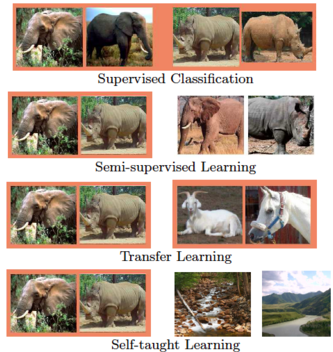
\includegraphics[width=2.8in]{selftaught.png}
\caption{Different learning setups}
\label{fig_sim}
\end{figure}


\subsubsection{Problem formulation}
Self-taught learning can be expressed as a two step optimization problem.

In the first step, the unlabeled data $x^{(i)}_u \in R^n, i=1..k$ is used to find a set of \textit{bases} $b_i \in R^n, i=1..s$ and a set of \textit{sparse activations} $a_j^{(i)}$ with $a^{(i)}\in R^s$ such that $x^{(i)}$ can
be reconstructed from the $s$ bases vectors $b$ and its corresponding activation weights $a^{(i)} \in R^s$ given by the formula:
\begin{equation}
\begin{array}{c }
	\min_{a,b} \sum_{i=1}^k ||x_u^{(i)} - \sum_j a_j^{(i)} b_j||_2^2 + \beta||a^{(i)}||_1    \\
	 s.t. ||b_j||_2 \leq 1, j=1..s
	\end{array}
\end{equation}
The equation above can be easily optimized using the algorithm from \cite{sparsetraining} by alternating the optimization in $a$ and $b$, e.g. fix one variable and optimize the other one at every step.
The problem is equivalent with a least square L1-regularized problem in variable $a$ and a least square constrained problem in  variable $b$. The L1-regularization enforces sparse representations and it was prefered to other forms of regulatization because experimentally it appeared to perform better across different datasets. We note that PCA can also be used for finding a new representation of the input, but it leads to different solutions for which the activations are linear combination of the input. Moreover,  PCA can not be used for generating more bases than the input dimension.


In the second step, the bases $b$ learned in the previous step are used for finding a higher level representation for labeled input data $x_l^{(i)}, i=1..m$ with corresponding target values $y_l^{(i)}, i=1..m$. The new representation given by the set of activation vectors $\hat{a}(x_l^{(i)}), i=1..m$ is obtained by solving another L1- regularized optimization problem:
\begin{equation}
\hat{a}(x_l^{(i)}) = \arg\min_{a^{(i)}}|| x_l^{(i)} - \sum_j a_j^{(i)}b_j||_2^2 + \beta||a^{(i)}||_1.
\end{equation}
As a last step, a classifier is trained on the pairs $\{\hat{a}(x_l^{(i)}), y^{(i)}\} , i=1..m$ and compared with a classifier (same type e.g. SVM) trained on the initial pairs $\{x_l^{(i)}, y^{(i)}\} i=1..m$.


\subsubsection{Experimental Results}
Self-taught learning was extensively tested across a range of different applications such as computer vision with raw pixel intensities as features, natural language processing with bag of words features and speech recognition with frequency histograms. Using an SVM as the classifier with sparse activation features as input instead of the initial raw features performed better in all except one tasks. This suggests that such a problem setup can be employed to datasets belonging to different domains besides the ones presented here.

\subsection{Information-Theoretic Regret Bounds for Gaussian Process Optimization in the Bandit Setting}

Many applications require the optimizion of a black box function $f: D\to R$ that is expensive to evaluate. Among them we mention: active user modelling, hierarchical reinforcement learning\cite{BPtutorial} and more recently, hyper parameter optimization of machine learning models \cite{hyperparameter}. This problem can be posed as a multi-armed bandit problem where the function to be estimated is sampled from a Gaussian Process.

The optimization is done in a sequential manner, where at round $t$ a point $x_t$ in the domain is chosen according to an \textit{acquisition function} and the value $f(x_t)$ is evaluated. The goal is to maximize f with as few samples as possible. Among the common used acquistion functions we note the Probabilty of Improvement, Maximum Expected Improvement or Upper Confidence Bound (called GP-UCB, the focus of this paper), with the latter two experimentally shown to perform better in practice. 

The effectiveness of a sampling scheme in finding the optimal $x* = \arg\max_{x\in D}f(x)$ ($x*$  may not be unique) is evaluated using the \textit{instantaneous} and the 
\textit{cumulative regret}.  The instantenous regret $r_t = f(x*) - f(x_t)$ is the error that we make at round t for choosing point $x_t$ instead of $x*$. The cumulative regret is the error accumulated up to the current round $R_T = \sum_{t=1..T} r_t$.

Besides the practical success of GP optimization, little was known in practice about its convergence properties for finite or infinte input dimensional space. The main contribution of the paper is to show sublinear convergence rates of the cumulative regret for GP-UCB in $T$, the number of rounds. In other words, as $T$ goes to infinity, we expect the cumulative regret to be 0: $\lim_{T\to\infty} \frac{R_T}{T} = 0$.

The bound on the cumulative regret $R_T$ is obtained in two steps. First bound $R_T$ using the information gain, then the information gain is bound using the empirical spectrum operator and the kernel operator spectrum.

\subsubsection{Gaussian Processes basics}
A Gaussian Process (GP) defines a distribution over functions $f$, $f \sim GP(u(x), k(x,x'))$, in a similar way in which probability densities define distributions over random variables. It is fully specified by its mean $u(x)$ and its covariance matrix $K$. In a Bayesian setting, we assume our function $f$ is sampled from a Gaussian with prior $GP(0, k(x,x'))$, where $k$ is the kernel or covariance matrix. The most common kernel types are the linear, squared exponential and Matern kernels.

For $T$ sampled points in the presence of noise, we have $y_t = f(x_t) + \epsilon_t$, where $\epsilon_t \in N(0,\sigma^2)$. The posterior over f, conditioned on $y_{1..T}$ and $x_{1..T}$ is given by
$P(f_T| y_{1:T},x_{1..T}) = N(u_T(x), \sigma_T^2(x))$, where: 
\begin{itemize}
	\item $K_T$ is positive definite with entries $k(x,x'), x,x' \in A_T$   
	\item $k_T(x) = [k(x_1,x),...k(x_T,x)]^T$	
	\item $k_{T}(x,x') = k(x,x') - k_T(x)^T(K_T+\sigma^2I)^-1k_T(x')$
	\item $u_{T}(x) = k_{T}(x)^{T}(K_T + \sigma^2I)^{-1} y_{T}$
	\item $\sigma_T^2(x) =  k_{T}(x,x)$
\end{itemize}

\subsubsection{Information Gain and Experimental Design}

Unlike function optimization where the goal is to find the maximum of a function, in experimental design the goal is to find a good approximation of the function globally with few samples as possible. We note that the same algorithm can not be employed for both tasks, since in function optimization we might want to avoid sampling in the regions where we are confident that the function has small values.

For a sampled set $x\in A$, we define $y_A = f_A + \epsilon_A$, where  $f_A=[f(x)]_{x \in A}$ and the noise $\epsilon_A \sim N(0,\sigma^2)$.
 The mutual information gain is
\begin{equation}
	I(y_A; f) = H(y_A) - H(y_A| f)
\end{equation}
where $H(y_A)$ and $H(y_A|f)$ represent the entropy or uncertainy in $y_A$ and 
the uncertainty in $y_A$ if we know f. In other words, information gain expresses the reduction in uncertainy about f given $y_A$.

Using the entropy formula for a Gaussian $H(N(u,\sigma)) =\frac{1}{2}log|2\pi e \Sigma|$ we can rewrite $F(A) =I(y_A; f)  = I(y_A; f_A) = \frac{1}{2} log|I + \sigma^{-2} K_A|$.
Finding the subset $A$ in the domain $D$ with $|A| \leq |T|$ that maximizes $I(y_A; f)$ is NP-hard. In practice, greedy approximation solutions are used that find a near-optimal solution by choosing a sequence of points in A with maximum variance at every step. Thus, the following equivalence relation holds at round t:
\begin{equation}
x_t = \arg\max_{x\in D} F(A_{t-1}\cup {x}) \Longleftrightarrow 
x_t = \arg\max_{x\in D}\sigma_{t-1}(x) 
\end{equation}
with $t\in{1...T}$

In \cite{nemhauser1978analysis} it is shown that for any submodular function $F(A)$ and set
$A_T$ obtained using the greedy aproach from above, it holds that:
\begin{equation}
	F(A_T) \geq (1-\frac{1}{e}) \max_{|A| \leq T}(F(A))
\end{equation}
Thus, a greedy set creation of $A_T$ leads to a solution close to the optimal.

\subsubsection{GP-UCB}
For the function optimization problem, a good sampling sequence $x_t$ is one that makes a tradeoff between 
exploration and exploitation of the search space. By choosing points with high variance (exploitation) we try to reduce the overall uncertainty.
By choosing points with high mean (exploration) we try to concentrate samples in a region were we are more confident that is close to the optimal. This idea is expressed by choosing in every round t, a point $x_t$  according to an acquistion function 
$x_t = \arg\max_{x\in D} u_{t-1} + \beta_{t}^{1/2}\sigma_{t-1}(x)$ with $\beta_{t}$ depending on the kernel type. The function that is being maximized is also called the acquistion function or utility function and corresponds to Upper Confidence Bound criterion.

To sum up, at every round, the GP-UCB algorithm selects a point according to the above equation, evaluates $y_t=f(x_t) + \epsilon$ and updates $u_t$ and $\sigma_t$ using Bayes rule.

An important property of the UCB defined as above is that it does not choose points $x_t$ for which the upper confidence value is smaller than the maximum lower confidence value found so far. This can prune large subareas of the search space.

\subsubsection{Regret Bounds}

This paper is the first to prove sublinear convergence rates for the cumulative regret $R_T$ with both finite and infinite input domain $D$ with smoothness assumptions on the kernel. The authors show that in the limit GP-UCB has no regret $\lim_{T\to\infty} \frac{R_T}{T}= 0$ and the convergence results for the most popular kernels can be found in table $I$, up to polylog factors. We notice that the dependance on the dimensionality $d$ of the input is weak. Namely, for the linear kernel the dependency is linear and for the squared exponential kernel $d$ appears only as a power of $log(T)$.
\begin{table}
\begin{tabular}{|c||c|c|c|}
\hline
Kernel & Linear & RBF & Matern\\
\hline
Regret $R_T$ & $d\sqrt{T}$& $\sqrt{T(log(T)^{d+1})} $ &${v+d(d+1)/2v+d(d+1)}$\\
\hline
\end{tabular}
\label{bounds}
\caption{Regret Bounds.}
\end{table}


\subsubsection{Bounding the Regret using Information Gain}
The first step of the proof is to bound $R_T$ by the maximum information gain $\gamma_T = \max_{A \subseteq D, |A| = T} I(y_A;f_A)$ after $T$ rounds.
In particular, it is shown that with high probability
\begin{itemize}
\item $Pr(R_T \leq \sqrt{C_1T\beta_T\gamma_T}) \leq 1- \delta$ for finite D
\item$Pr(R_T \leq \sqrt{C_2T\beta_T\gamma_T} + 2) \leq 1- \delta$ for  D compact and convex 
\end{itemize}
where $\delta \in (0,1)$ and appropiate constants $C_1, C_2, \beta_t$ . The second inequality holds by making further assumptions that the function is smooth, e.g. by enforcing that the probability of the partial derivatives of the function to have a large value is small.

\subsubsection{Bounding the Information Gain using the empiricial spectrum}
The case of  infinite input dimensionionality are treated similarly with the finite case by assuming the existence of a discretized set $D_T \subset D, T \in N $ with nearest neighbor distance O(1), dense in the limit. As stated previously, the value of $\gamma_T= \max_{A\subset D_T, |A|=T} I(y_A; f_A)$ can be bounded by the greedy maximization value $ \gamma_T \leq \frac{1}{1-e^{-1}} F(A_T)$ since it is a submodular function. 

Choosing a point $x_t$ is equivalent with selecting a vector $v_t\in R^{|D|}$ with values 0's except the entry at position $t$, thus $f\sim N(v_tf,\sigma^2)$. By relaxating the constraint to $||v_t|| = 1$, it is shown that the $v_t$'s are selected among the eigenvectors of the kernel matrix $K_{D_T} = k(x,x'),  x,x' \in D_T$. The maximum information gain is further bounded by an expression involving the eigenvalues $\hat{\lambda_t}$ of $K_{D_T}$ as follows:		
\begin{equation}		
	\gamma_T \leq \frac{0.5}{1-e^{-1}} \max_{m_1,m_2,...,m_D} \sum_{t=1}^{|D|} log(1 + \sigma^{-2}m_t \hat{\lambda_t})		
\end{equation}		
where $m_t\in N$, $\sum_t m_t = T$ and $\hat{\lambda_1} \geq \hat{\lambda_2} \geq \hat{\lambda_3} \geq ..$. Here a worst case scenario was considered for assigning eingevectors of $K_T$ to $v_t$.			
In the next step, the information gain is bounded using the tail spectrum of $K_{D_T}$, $B(T_{*}) = \sum_{t=1}^{T_*}\hat{\lambda_t}$ and $n_T = \sum_{t=1}^{T_*} \hat{\lambda_t}$ for any $T_{*}=1..T$:		
\begin{equation}		
\gamma_{T} \leq O(\sigma^{-2}[B(T_{*})T + T_{*}logn_T T)])		
\end{equation}		
		
From the equation above, we conclude that if the tail spectrum $B(T_{*})$ is small, or in others words, the eingenspetrum of $K_{D_T}$ decays fast, the bound on $\gamma_T$ is tighter.		
\subsubsection{Bounding the empirical spectrum by the operator spectrum}		
For a kernel k with $\int k(x,x)u(x)=1$ where u(x) is uniformly distributed on $D$, Mercer's theorem assures the existence of a discrete kernel eigenspectrum $\{\lambda_s(x), \phi_s(x) \}$		
with $k(x,x') = \sum \lambda_s\phi_s(x) \phi_s(x')$		
		
Another contribution(?) of this paper is to bound the empirical tails spectrum $B(T_{*})$ by the kernel operator tails eigenspectrum $B_k(T_{*}) = \sum_{t=1}^{T_*}\lambda_t $. Analytical expression bounds on $B_k(T_{*})$ for the most common kernels are given by Seeger \cite{NonGP}.		
		
\subsubsection{Conclusions}		
The contribution of the paper is two fold. First, a novel connection was made between experimental design and GP optimization, by bounding the cumulative regret by the maximum information gain. Secondly, sublinear regret bounds for GP-UCB optimization are shown with weak dependence on the dimensionality of the input for the first time. 		
 The bound is derived in two steps. First, the cumulative regret is bounded by the maximum information gain which in turn is bounded by the tails of the empirical eigenspectrum and the kernel operator spectrum. The thighter the bound is, the more rapidly the kernel spectrum decays. 

Although convergence rates are proven for infinite input dimensional spaces as well, the complexity of the GP step that incorporates the inversion of the covariance matrix makes the complexity of the algorithm cubic in the number of samples T, which makes it often impractical for high dimensional input.

\section{Research Proposal}
\subsection*{•}
I propose a new descriptor that is more robust to atom indexing, called Bag of Bonds Histogram (BoBH). Its size is not dependent on the number of atoms in a molecule but on the number of different atom types. Every bag in a BoBH descriptor is a histogram of quantized distances which encodes information for all pairs of atoms of same composition. The size of the histogram bag is given by the maximum distance between two pairs of atoms (pertaining to that bag type). The quantization level of the distances varies between bag types and we experimentally found that a quantization level of 0.2 or 0.25 perform well in practice, but this can vary for different datasets.

Thus, for a given molecule, the BoBH descriptor will encode:
\begin{itemize}
\item 
for every different atom type present in the dataset, how many times it appears in the molecule
\item  
for every pair of atoms of certain type, how many times the distance between them is in a given quantization interval 
\end{itemize}

An example is given in Fig \ref{fig:BoBH} for a molecule $C_{4}H_{2}O$ with a quantization level of $q=1$. In this example, first the bags containing H were concatenated, then the ones containing C and in the end the ones containing O, resulting in a descriptor of size 21. In general, the size of the descriptor is given by $NA + \sum_i \frac{N_A*(N_A+1)}{2} *\frac{D_{max}}{q} $, where $N_A$ is the number of atom types and $D_{max}$ is the maximum distance between a pair of atoms. 

\begin{figure}[h!]

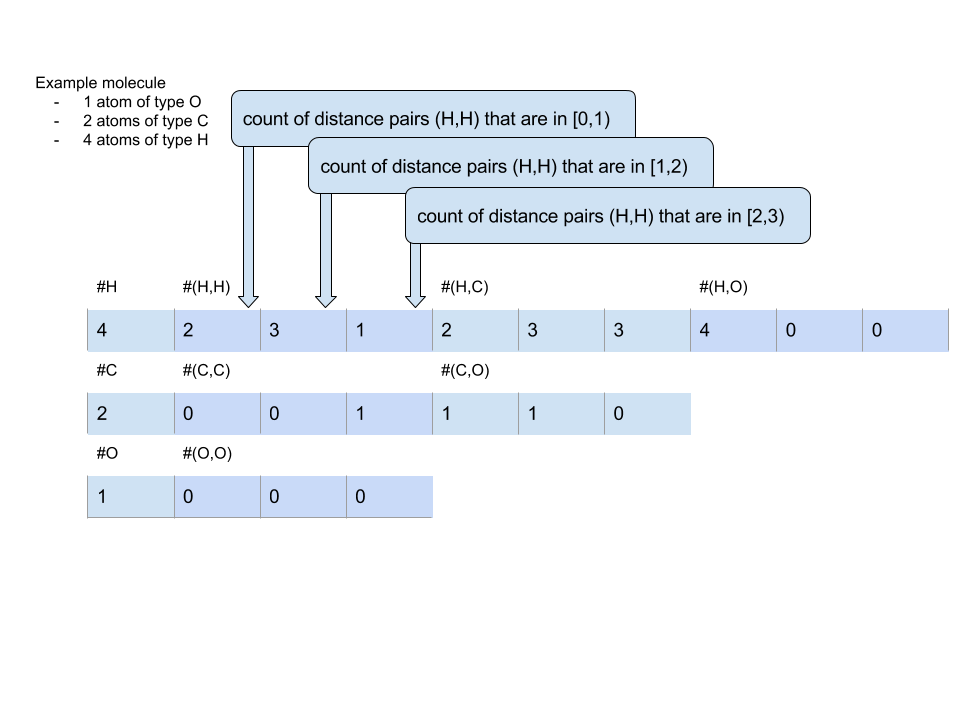
\includegraphics[scale=0.25]{HistogramOfDistances.png}
\caption{Bag of Bonds Histogram.
Sample computation of Bag of Bonds Histogram for $C_2H_4O$ for a dataset which contains only atoms of type O, C and H. If the maximum distance between any two atoms in our dataset is 3, the size of the BoBH descriptor with quantization level  1 is 21, as shown above. The first entry encodes the number of H atoms, 4. The following 3 elements encode the number of (H,H) distances that fall in the interval [0,1), [1,2) and [2,3).
}
\label{fig:BoBH}
\end{figure}


To sum up, molecular descriptors achieve translation and rotation invariance through the use of
distances between atoms instead of the actual 3D positions. Sorted Coloumb and Randomly Sorted Coloumb achieve invariance to index permutation by sorting the rows of the matrix according to their norm. Bag of Bonds Histogram places atom pairs with the same composition in the same bag and quantizes the distances into bins to bypass the sorting step. Preliminary results on the same dataset as in \cite{montavon2012learning}  show promising results, obtaining a MAE of 2.6 kcal/mol.

\subsection*{•}
Another issue that we would like to address is the fact the preprocessing the molecular data to be used in a machine learning setting requires extensive domain specific knowledge. As an example, generating the folds for cross validation using stratified sampling is a good strategy for obtaining good generalization performance but in practice, we should not expect to know the range of the test data. If we test the performance on a new molecule whose atomization energy is not within the bounds present in the training dataset, it is likely that the prediction will not be very accurate. Moreover, if we have a molecule with more atoms than any molecule present in the dataset, we would need to retrain our model with a  descriptor of different size. 

The same problem appears across chemical compound space if we try to predict the atomization energy of a molecule with the same number of atoms but with different atom types in its composition. In general, we do not have guarantees that a molecule with similar atom composition and similar atom type have target prediction in the same range as our training set.

The labeled datasets\footnote{All datasets can be downloaded from \textit{www.quantum-mechanics.org}} currently used  are in the order of 7k or 140k samples and are of relatively small size compared with datasets sizes in other domains. Specifically, they contain at most 6 atom types and at most 29 atoms per molecule. In chemoinformatics, the datasets can not be easily augumented by using external annotation tools since it requires domain knowledge and the labeling effort implies time intensive computations.

One proposed solution to the above issues is to use large amounts of unlabeled data as in \cite{selftaughtl}.
Although the self-taught learning problem in \cite{selftaughtl} was tested only for classification tasks and predicting properties of molecules is a regression task, employing large amounts of unlabeled molecular data for obtaining higher level representations of the molecules has the potential of increasing performance results across datasets by avoiding the labeling effort.


%Propose of augumententing the data sets more easily and make the cross validation
%less sensitive to splitting -at the moment : take non H atoms, then sort then do CV.
%
%MOVE thIS The more available labeled data, the use of the unlabeled data becomes less important.

In other words, our problem can be formulated as a semi-supervised, transfer-learning or self-taught learning problem by making it generalize across chemical compound space and learn new embeddings of the molecules. As an example, we could try to learn a set of bases features from one dataset containing $\{H, C, O, S, N\}$ and use this representation for a new set containg $\{H, C, O, S, Cl\}$.\\[0.05in]



Another problem we would like to investigate is the difficulty in training neural networks. The authors of \cite{montavon2012learning} make use of various tricks \cite{tricks} to obtain state-of-the-art performance on the molecular datasets. A grid search approach for choosing the hyper parameters of a model leads to exponential time complexity in the number of parameters.
Recent work \cite{hyperparameter}, \cite{citeulike} suggests the use of Bayesian optimization techniques (such as GP-UCB or Bayesian neural networks) for hyper-parameters tuning. In this setup, the function to be maximized is the accuracy on the validation set while the input represents the concatentation of the hyper parameters (learning rate, type of activation function, number of units per hidden layer etc.). The speedup in training time can be quite significant, since techniques such as GP-UCB employ an exploration - exploitation trade-off scheme that prunes large areas of the search space.
In \cite{citeulike} they experimentally demonstrate on a NLP task, that by using a simple model tuned in a Bayesian optimizatin setting can outperform the use of a more complex model (such as Recurrent Neural Networks).
Such techniques which were sucessfully applied for fine tuning NLP and vision models can be employed to molecular models as well.
One further direction that can be followed is to try to reach the desired chemical accuracy level of prediction of $\sim 1kcal/mol$ MAE for atomization energy by fine-tuning existing models using Bayesian optimization techniques. 
Since this will allow us to search over a larger space of models with a reduced computational search compared to grid search, we would like to investigate the potential of reaching state-of-the-art performance combining existing setups and descriptors.

%Talk if we have time about bayesian neural nets, were simpler models outperform more easy models just be using hyper parameter optimization instead of grid search.

% \textcolor{blue}{Write how you
%propose to advance the state of the art given the background. What
%is new technically? How does it improve over prior work?
%Summarize, suggest an approximate timeline, and list references.}
% In our scenario, this can be used for
%tuning the hyper-parameters of the model trained.
%Here the input dimensionality is given by the nbr of the hyper parameters (learning rate, activation fct, nbr hidden layers) used and the fct to be minimized is the cross validation error.
%Although the use of Gaussian processes in material design is not new, it s major drawback is the computational bottleneck.
%The result presented in the previous subsection were obtained like that.
\vspace{1cm}



% trigger a \newpage just before the given reference
% number - used to balance the columns on the last page
% adjust value as needed - may need to be readjusted if
% the document is modified later
%\IEEEtriggeratref{8}
% The "triggered" command can be changed if desired:
%\IEEEtriggercmd{\enlargethispage{-5in}}

% references section

% can use a bibliography generated by BibTeX as a .bbl file
% BibTeX documentation can be easily obtained at:
% http://www.ctan.org/tex-archive/biblio/bibtex/contrib/doc/
% The IEEEtran BibTeX style support page is at:
% http://www.michaelshell.org/tex/ieeetran/bibtex/
%\bibliographystyle{IEEEtran}
% argument is your BibTeX string definitions and bibliography database(s)
%\bibliography{IEEEabrv,../bib/paper}
%
% <OR> manually copy in the resultant .bbl file
% set second argument of \begin to the number of references
% (used to reserve space for the reference number labels box)


% biography section
% 
% If you have an EPS/PDF photo (graphicx package needed) extra braces are
% needed around the contents of the optional argument to biography to prevent
% the LaTeX parser from getting confused when it sees the complicated
% \includegraphics command within an optional argument. (You could create
% your own custom macro containing the \includegraphics command to make things
% simpler here.)
%\begin{biography}[{\includegraphics[width=1in,height=1.25in,clip,keepaspectratio]{mshell}}]{Michael Shell}
% or if you just want to reserve a space for a photo:

%\begin{IEEEbiography}{Michael Shell}
%Biography text here.
%\end{IEEEbiography}

% if you will not have a photo at all:
%\begin{IEEEbiographynophoto}{John Doe}
%Biography text here.
%\end{IEEEbiographynophoto}

% insert where needed to balance the two columns on the last page with
% biographies
%\newpage

%\begin{IEEEbiographynophoto}{Jane Doe}
%Biography text here.
%\end{IEEEbiographynophoto}

% You can push biographies down or up by placing
% a \vfill before or after them. The appropriate
% use of \vfill depends on what kind of text is
% on the last page and whether or not the columns
% are being equalized.

%\vfill

% Can be used to pull up biographies so that the bottom of the last one
% is flush with the other column.
%\enlargethispage{-5in}



\bibliographystyle{plain}
\bibliography{references}
\end{document}


